\documentclass[12pt, a4paper]{article}

\usepackage[utf8]{inputenc}
% Limit the page margin to only 1 inch.
\usepackage[margin=1in]{geometry}

%Imports biblatex package
\usepackage[
backend=biber,
style=alphabetic
]{biblatex}
\addbibresource{../../algs4e.bib}

% Enables the `align' environment.
\usepackage{amsmath}
% Provides useful environments, such as:
% - \begin{proof} ...\end{proof}
\usepackage{amsthm}
\usepackage[most]{tcolorbox}

\newtheorem*{proposition}{Proposition}

% Enables using \mathbb{}, for example \mathbb{N} for the set of natural numbers.
\usepackage{amssymb}

% Allows using letters in enumerate list environment. Use, for example:
%\begin{enumerate}[label=(\alph*)]
% ...
%\end{enumerate}
\usepackage[inline]{enumitem}

% Enable importing external graphic files and provides useful commannds, like \graphicspath{}
\usepackage{graphicx}
% Images are located in a directory called images in the current directory.
\graphicspath{{./images/}}

% Make links look better by default.
% See: https://tex.stackexchange.com/questions/823/remove-ugly-borders-around-clickable-cross-references-and-hyperlinks
\usepackage[hidelinks]{hyperref}
\usepackage{xcolor}
\hypersetup{
	colorlinks,
	linkcolor={red!50!black},
	citecolor={blue!50!black},
	urlcolor={blue!80!black}
}


% Code Listings. Source:
% https://stackoverflow.com/questions/3175105/inserting-code-in-this-latex-document-with-indentation
\usepackage{listings}
\usepackage{color}

\definecolor{dkgreen}{rgb}{0,0.6,0}
\definecolor{gray}{rgb}{0.5,0.5,0.5}
\definecolor{mauve}{rgb}{0.58,0,0.82}

\lstset{frame=tb,
	language=Java,
	aboveskip=3mm,
	belowskip=3mm,
	showstringspaces=false,
	columns=flexible,
	basicstyle={\small\ttfamily},
	numbers=none,
	numberstyle=\tiny\color{gray},
	keywordstyle=\color{blue},
	commentstyle=\color{dkgreen},
	stringstyle=\color{mauve},
	breaklines=true,
	breakatwhitespace=true,
	tabsize=3
}

\newcommand{\prob}{\text{P}}
%\newcommand{\complement}{\mathsf{c}}

% Define an environment called "ex" (for Exercise) so that I can do: \begin{ex}{1.5}...\end{ex}
\newenvironment{ex}[2][Exercise]
{\par\medskip\noindent \textbf{#1 #2.}}
{\medskip}

% Define a solution environment, similar to ex (exercise) environment.
\newenvironment{sol}[1][Solution]
{\par\medskip\noindent \textbf{#1.} }
{\medskip}

\begin{document}
	\noindent Sergio E. Garcia Tapia \hfill
	
	\noindent \emph{Algorithms} by Sedgewick and Wayne (4th edition) \cite{sedgewick_wayne}\hfill
	
	\noindent December 31st, 2024\hfill 
	\section*{3.3: Balanced Search Trees}
	\begin{ex}{1}
		Draw the 2-3 tree that results when you insert the keys \texttt{E A S Y Q U T I O N}
		in that order into an initially empty tree.
	\end{ex}
	\begin{sol}
		See Figure~\ref{fig:ex-01}
		\begin{figure}
			\centering
			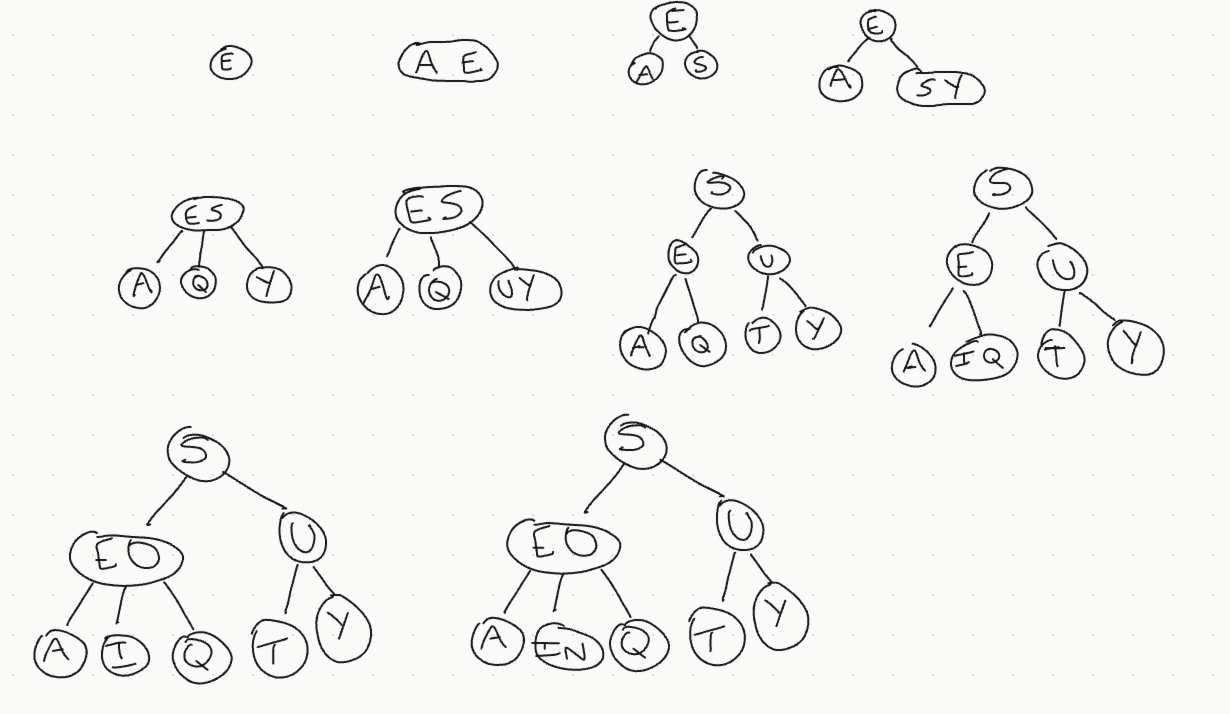
\includegraphics[width=0.7\textwidth]{exercise-01}
			\caption{Sequence of 2-3 trees when inserting the keys in Exercise 1.}
			\label{fig:ex-01}
		\end{figure}
	\end{sol}
	\begin{ex}{2}
		Draw the 2-3 tree that results when you insert the keys
		\texttt{Y L P M X H C R A E S} in that order into an initially empty tree.
	\end{ex}
	\begin{sol}
		See Figure~\ref{fig:ex-02}
		\begin{figure}
			\centering
			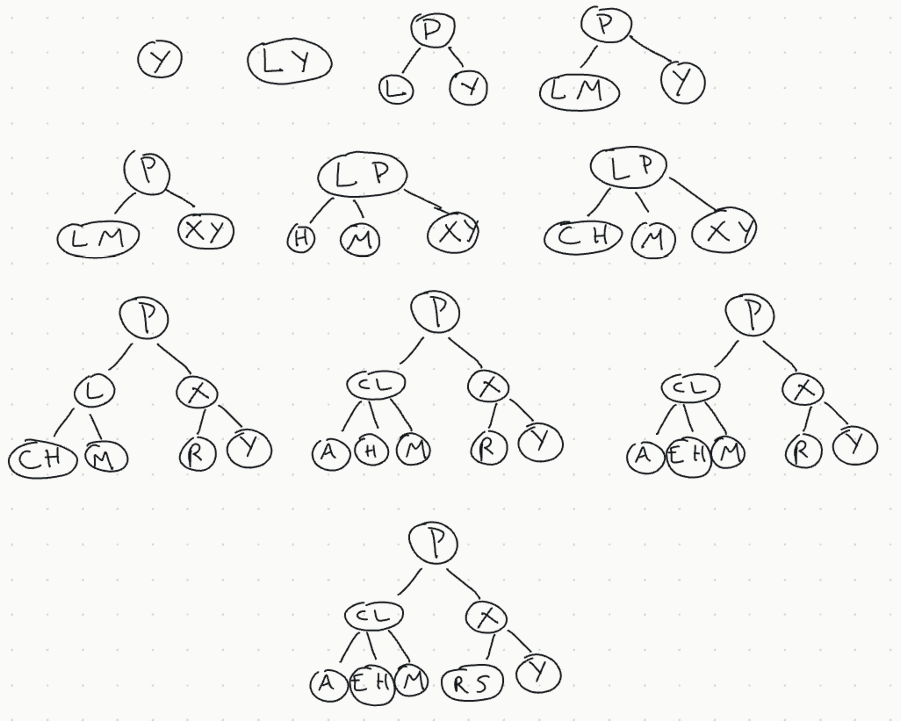
\includegraphics[width=0.6\textwidth]{exercise-02}
			\caption{Sequence of 2-3 trees when inserting the keys in Exercise 2.}
			\label{fig:ex-02}
		\end{figure}
	\end{sol}
	\begin{ex}{3}
		Find an insertion order for the keys \texttt{S E A R C H X M} that leads to a
		2-3 tree of height 1.
	\end{ex}
	\begin{sol}
		See Figure~\ref{fig:ex-03}.
		
		\begin{figure}
			\centering
			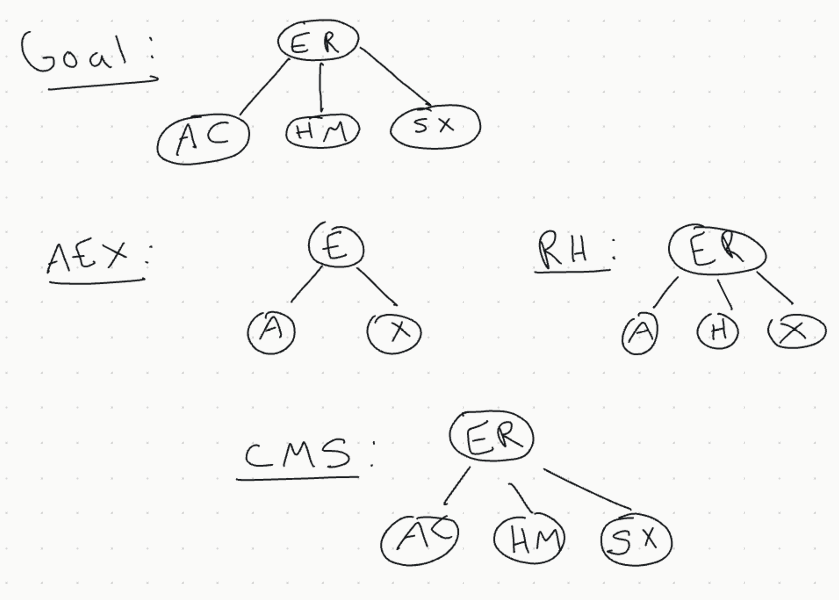
\includegraphics[width=0.6\textwidth]{exercise-03}
			\caption{Tree of height 1 for keys in Exercise 3.}
			\label{fig:ex-03}
		\end{figure}
		
		First, consider the the sort of the keys is \texttt{A C E H M R S X}.
		Since there are 8 keys, we can obtain a tree of height 1 if we have four 3-nodes.
		In particular, \texttt{E} and \texttt{R} are at the root, and \texttt{A} and \texttt{X}
		are in the leftmost and rightmost leaves, respectively. We can begin by inserting
		\texttt{AEX}, which places \texttt{E} at the root as desired. We can then insert
		\texttt{R} and \texttt{H}. Both fall in the rightmost leaf, and the split of the
		4-node that is created causes \texttt{R} to move to the root node, and the
		creation of the new leaf \texttt{H}. Now inserting \texttt{C} yields the 3-node
		with \texttt{A} and \texttt{C}, inserting \texttt{M} yields the node with \texttt{H} and
		\texttt{M}, and inserting \texttt{S} yields the node with \texttt{S} and \texttt{X}.
	\end{sol}
	\begin{ex}{4}
		Prove that the height of a 2-3 tree with $n$ keys is between $\lfloor \log_3n\rfloor
		\approx 0.63\lg n$ (for a tree that is all 3-nodes) and $\lfloor \lg_n\rfloor$
		(for a tree that is all $2$-nodes).
	\end{ex}
	\begin{sol}
		\begin{proof}
			Suppose $T$ is a 2-3 search tree. By construction, a 2-3 search tree is
			perfectly balanced, so $T$ is perfectly balanced also. In the worst case, if
			$T$ consists of only 2-nodes, then it will have $2^k$ nodes at all depths
			(except possibly the last one) because it is balanced. Similarly, in the best
			case, if $T$ consists only of 3-nodes then it will have $3^k$ nodes at all
			depths (except possibly the last one). The former tree has a height of
			$\lfloor \lg_n\rfloor$, and the latter has a height of $\lfloor \log_3 n\rfloor$.
			We conclude that $T$'s height lies in between the two.
		\end{proof}
	\end{sol}
	\begin{ex}{5}
		Figure~\ref{fig:ex-05-1} shows all the \emph{structurally different} 2-3 trees with $n$
		keys, for $n$ from 1 up to 6 (ignore the order of the subtrees). Draw all the structurally
		different trees for $n=$ $7$, $8$, $9$, and $10$.
		\begin{figure}
			\centering
			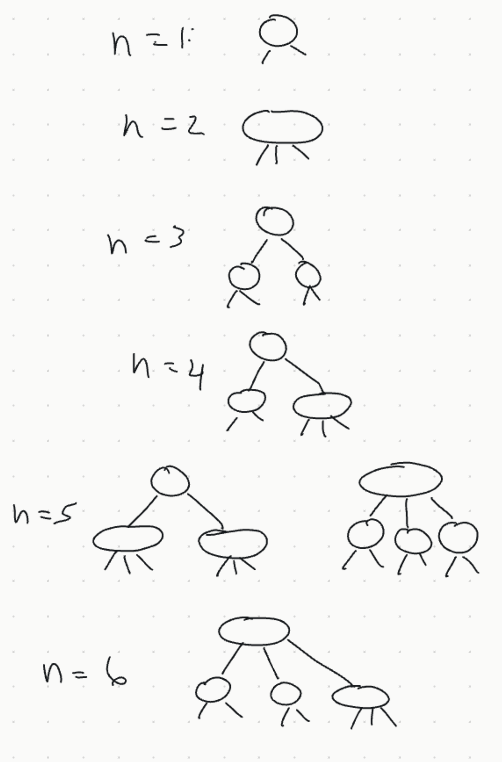
\includegraphics[width=0.4 \textwidth]{exercise-05-1}
			\caption{All of the structurally different 2-3 trees with $n$ keys, for
			$n$ from 1 through $6$.}
			\label{fig:ex-05-1}
		\end{figure}
	\end{ex}
	\begin{sol}
		See Figure~\ref{fig:ex-05-2}.
		\begin{figure}
			\centering
			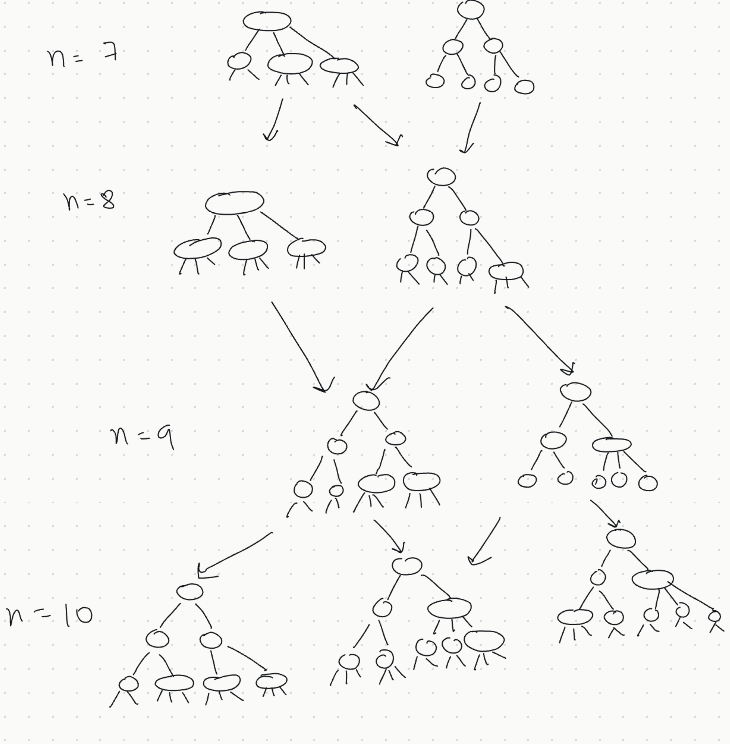
\includegraphics[width=0.6\textwidth]{exercise-05-2}
			\caption{All of the structurally different 2-3 trees with $n$ keys, for
				$n$ from $7$ through $10$.}
			\label{fig:ex-05-2}
		\end{figure}
	\end{sol}
	\begin{ex}{6}
		Find the probability that each of the 2-3 trees in Exercise 3.3.5 is the result
		of the insertion of $n$ random distinct keys into an initially empty tree.
	\end{ex}
	\begin{sol}
		See Figure~\ref{fig:ex-06-1} and Figure~\ref{fig:ex-06-2}, both of which I
		have annotated. Note that when a given tree can lead to more than one structurally
		different tree, I have annotated the arrows indicating the probability with
		which it can give rise to said structure. This ``transitional probability"
		then plays a role in the computation of the probabilities of the resulting tree.
		\begin{figure}
			\centering
			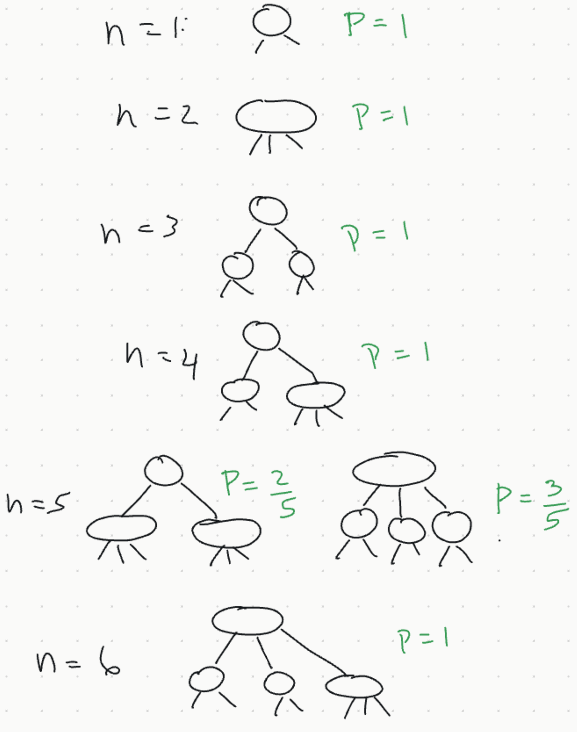
\includegraphics[width=0.6\textwidth]{exercise-06-1}
			\caption{All of the structurally different 2-3 trees with $n$ keys, for
				$n$ from $1$ through $6$ and their probabilities.}
			\label{fig:ex-06-1}
		\end{figure}
		\begin{figure}
			\centering
			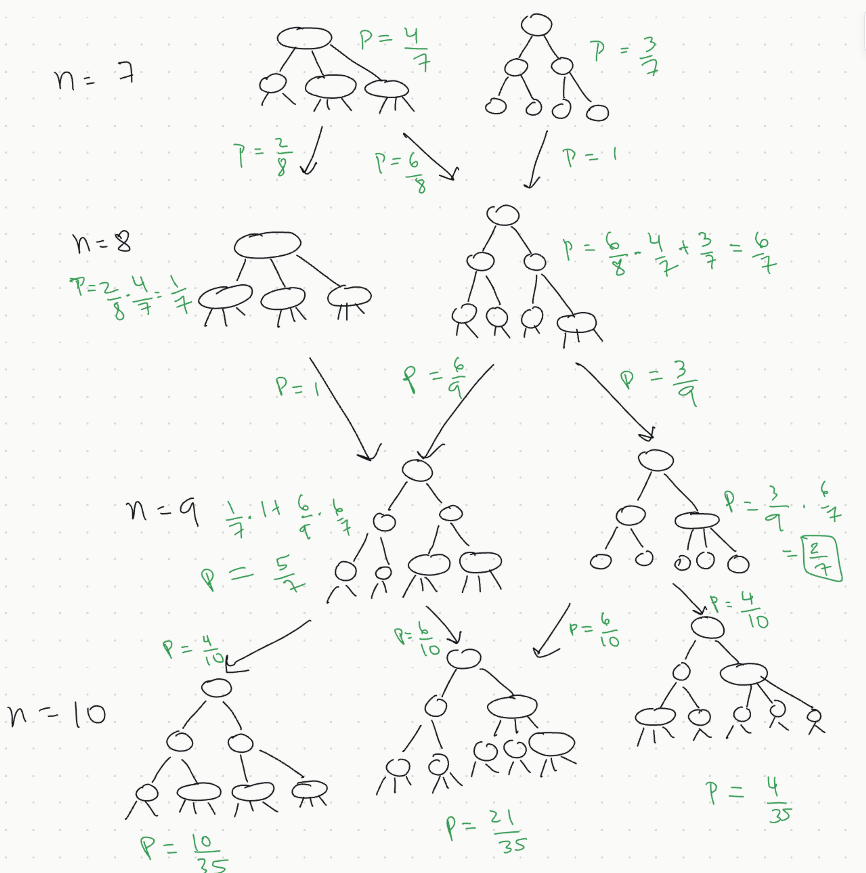
\includegraphics[width=0.7\textwidth]{exercise-06-2}
			\caption{All of the structurally different 2-3 trees with $n$ keys, for
				$n$ from $7$ through $10$ and their probabilities.}
			\label{fig:ex-06-2}
		\end{figure}
	\end{sol}
	\begin{ex}{8}
		Show all possible ways that one might represent a 4-node with three 2-nodes
		bound together with red links (not necessarily left-leaning).
	\end{ex}
	\begin{sol}
		See Figure~\ref{fig:ex-08}.
		\begin{figure}
			\centering
			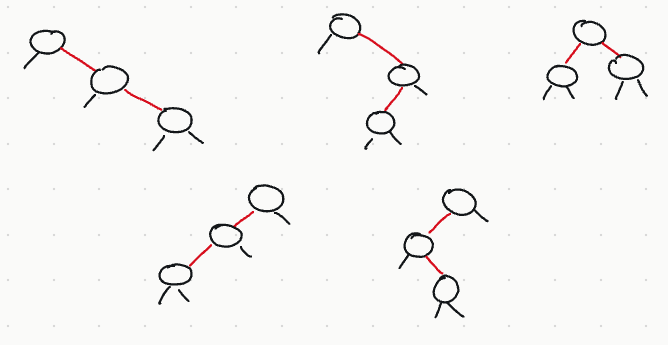
\includegraphics[width=0.6\textwidth]{exercise-08}
			\caption{All ways to represent a 4-node with three 2-nodes bound by red links.}
			\label{fig:ex-08}
		\end{figure}
	\end{sol}
	\begin{ex}{9}
		Which of the trees in Figure~\ref{fig:ex-09} are red-black BSTs?
		\begin{figure}
			\centering
			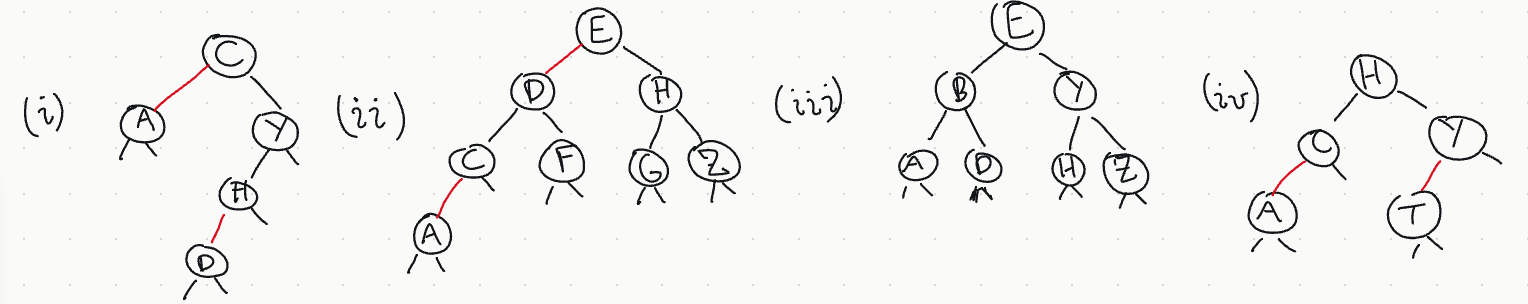
\includegraphics[width=0.9\textwidth]{exercise-09}
			\caption{Options for Exercise 9.}
			\label{fig:ex-09}
		\end{figure}
	\end{ex}
	\begin{sol}
		 Tree (i) is not a red-black BST because it does not have perfect black balance.
		 Tree (ii) is not a red-black BST because it is not ordered. In particular,
		 \texttt{F} is on the left subtree of \texttt{E} instead of right. The remaining
		 trees are red-black BSTs.
	\end{sol}
	\begin{ex}{10}
		Draw the red-black BST that results when you insert items with the keys
		\texttt{E A S Y Q U T I O N} in that order into an initially empty tree.
	\end{ex}
	\begin{sol}
		 See Figure~\ref{fig:ex-10}.
		 \begin{figure}
		 	\centering
		 	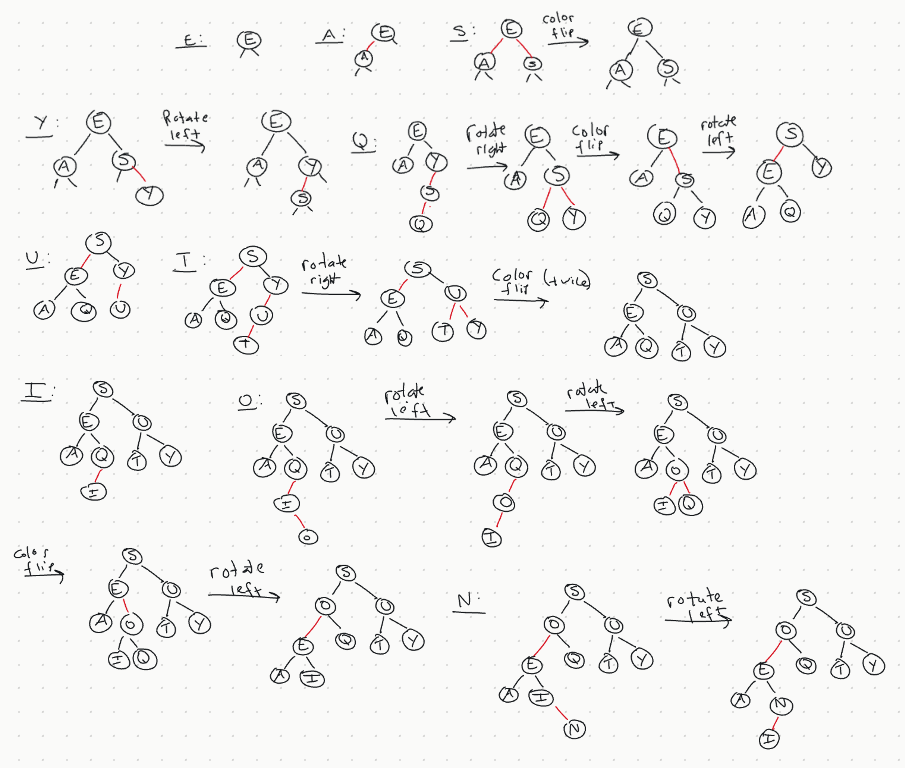
\includegraphics[width=0.9\textwidth]{exercise-10}
		 	\caption{Sequence of red-black BSTs generated by the key sequence in Exercise 10.}
		 	\label{fig:ex-10}
		 \end{figure}
	\end{sol}
	\begin{ex}{11}
		Draw the red-black BST that results when you insert the keys
		\texttt{Y L P M X H C R A E S} in that order into an initially empty tree.
	\end{ex}
	\begin{sol}
		By using the 1-1 corresponding of 2-3 trees and red-black BSTs, we can use the 2-3
		tree in Exercise 3.3.2 to create the corresponding red-black BST, depicted
		in Figure~\ref{fig:ex-11}.
		\begin{figure}
			\centering
			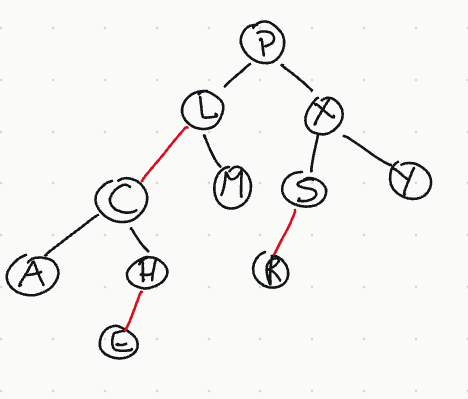
\includegraphics[width=0.4\textwidth]{exercise-11}
			\caption{Red-black BST resulting from the key sequence in Exercise 11.}
			\label{fig:ex-11}
		\end{figure}
	\end{sol}
	\begin{ex}{13}
		True or false: If you insert keys in increasing order into a red-black BST, the tree
		height is monotonically increasing.
	\end{ex}
	\begin{sol}
		True. Because the keys are inserted in increasing order, they always fall on the rightmost
		child of the rightmost leaf. However, such a tree would have a right-leaning red link,
		so it is rotated left to complete the insertion. When the link is rotated left, the height
		remains unaffected.
		
		As the insertions continue, there will never be a tree with two consecutive right-leaning
		links, because the previous insertion would rotate the link left. We will have
		to perform color flips, but they do not change the height either. The color flips will create
		new right-leaning red links, which may need to be handled by rotation, but the tree
		height is not decreased as a result of this.
		
		One effect that color flips have, however, is that because they always occur
		in a right subtree (due to the pattern of inserting keys in increasing order),
		they will create right-leaning red links. When these occur further up the tree,
		there is potential for them to decrease the tree height. However, this does not happen
		because when they occur the subtrees differ by height of 1 (with the right
		subtree being the larger), so the rotation to the left does not affect the overall
		tree height.
	\end{sol}
	\begin{ex}{14}
		Draw the red-black BST that results when you insert letters \texttt{A} through
		\texttt{K} in order into an initially empty tree, then describe what happens in general
		when trees are built by insertion of keys in ascending order.
	\end{ex}
	\begin{sol}
		See Figure~\ref{fig:ex-14}
		\begin{figure}
			\centering
			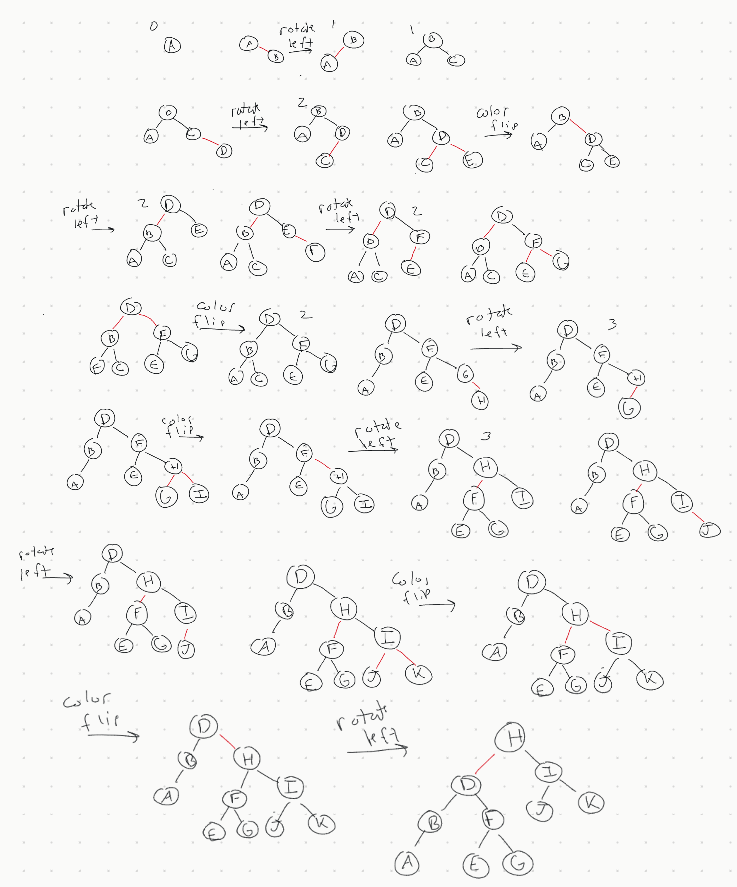
\includegraphics[width=0.8\textwidth]{exercise-14}
			\caption{Inserting keys in decreasing order into a red-black BST.}
			\label{fig:ex-14}
		\end{figure}
		See the explanation in Exercise 13.
	\end{sol}
	
	\begin{ex}{15}
		Answer the previous two questions for the case when the keys are inserted in \emph{descending}
		order.
	\end{ex}
	\begin{sol}
		The tree height is not monotonically increasing.
		\begin{figure}
			\centering
			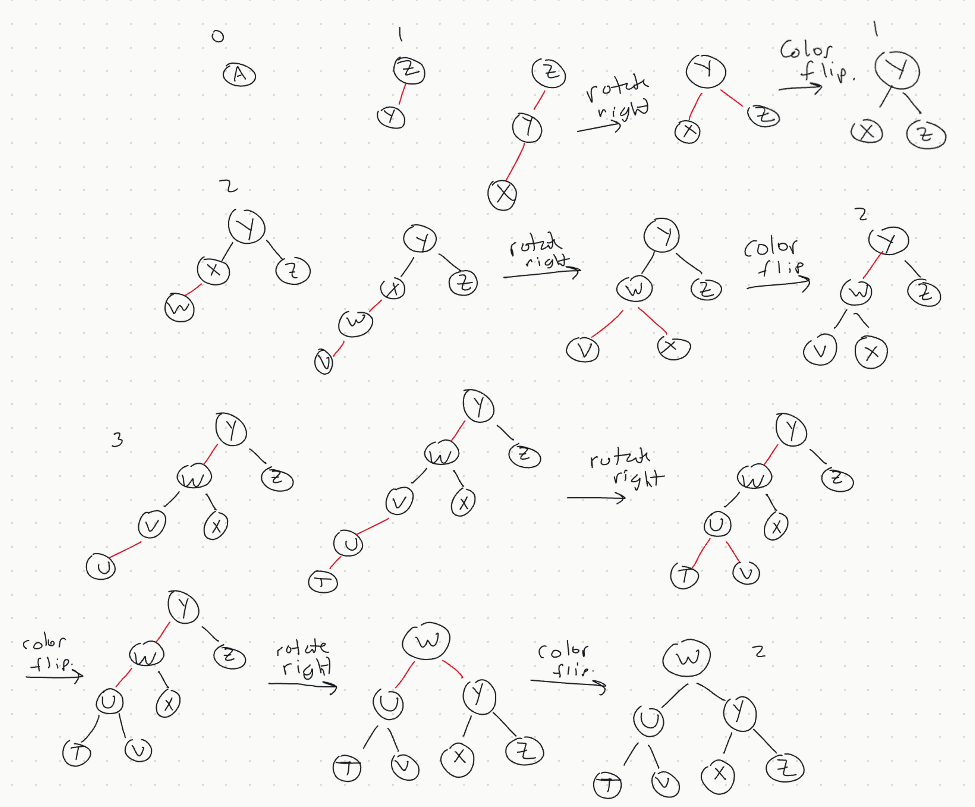
\includegraphics[width=0.8\textwidth]{exercise-15}
			\caption{Inserting keys in decreasing order into a red-black BST.}
			\label{fig:ex-15}
		\end{figure}
		In Figure~\ref{fig:ex-15}, we see that after \texttt{T} is inserted, the sequence
		of transformations takes us from a tree of height 3 to a tree of height 2. The
		reason is that since left-leaning red links are valid, they are allowed to remain.
		Since all insertions result in left-leaning red links, we will often encounter two
		consecutive left-leaning red links, which must be handle via a right rotation.
		At the bottom of a tree, this does not affect the height. However, the further
		rotations triggered can change the height, such as the one happening at the
		root in the figure. There, the rotation makes \texttt{W} the root, and the
		leaves of greatest depth in the tree are the leaves in \texttt{W}'s subtree.
		The rotation decreases their depth by 1, and hence the height of the
		overall tree.
	\end{sol}
	\begin{ex}{20}
		Compute the internal path length in a perfectly balanced BST of $n$ nodes, when
		$n$ is a power of 2 minus 1.
	\end{ex}
	\begin{sol}
		Let $n=2^m-1$. Then the BST has height $m-1$. Such a tree is a perfect binary tree.
		At depth $k$ there are $2^k$ nodes, so the internal path length is
		\begin{align*}
			\sum_{k=0}^{m-1}k\cdot 2^k
		\end{align*}
	\end{sol}
	\begin{ex}{23}
		\emph{2-3 trees without balance restriction}. Develop an implementation of the basic
		symbol-table API that uses 2-3 trees that are not necessarily balanced as the underlying
		data structure. Allow 3-nodes to lean either way. Hook the new node onto the bottom
		with a \emph{black} link when inserting into a 3-node at the bottom. Run experiments
		to develop a hypothesis estimating the average length in a tree built from $n$ random
		insertions.
	\end{ex}
	\begin{sol}
		See \texttt{com.segarciat.algs4.ch3.sec3.ex23.TwoThreeST}.
	\end{sol}
	\begin{ex}{25}
		\emph{Top-down 2-3-4 trees}. Develop an implementation of the basic symbol-table API
		that uses balanced 2-3-4 trees as the underlying data structure, using the red-black
		representation and the insertion method described in the text, where 4-nodes are split
		by flipping colors on the way down the search path and balancing on the way up.
	\end{ex}
	\begin{sol}
		See \texttt{com.segarciat.algs4.ch3.sec3.ex25.TwoThreeFourST}
	\end{sol}
	\begin{ex}{26}
		\emph{Single top-down pass}. Develop a modified version of your solution to
		\textbf{Exercise 3.2.25} that does \emph{not} use recursion. Complete all the work
		splitting and balancing 4-nodes (and balancing 3-nodes) on the way down the tree,
		finishing with an insertion at the bottom.
	\end{ex}
	\begin{sol}
		See \texttt{com.segarciat.algs4.ch3.sec3.ex26.TwoThreeFourST}
	\end{sol}
	\begin{ex}{31}
		\emph{Tree drawing}. Add a method \texttt{draw()} to \texttt{RedBlackBST} that
		draws red-black BST figures in the style of the text (see \textbf{Exercise 3.2.38}).
	\end{ex}
	\begin{sol}
		See \texttt{com.segarciat.algs4.ch3.sec3.ex31.RedBlackBST}
	\end{sol}
	\begin{ex}{32}
	\end{ex}
	\begin{sol}
		\begin{proof}
			First we can show that the coloring yields a 2-3-4 tree. Say we color
			red any link from a node of even height to a node of odd height.
			There are five cases:
			\begin{enumerate}
				\item If a node has odd height, then the parity of the height of
				the children is irrelevant; the links to these nodes are black,
				so the node is a 2-node.
				\item If a node has even height and both of its children are of
				even height, then the links to these nodes is black, making
				the current node a 2-node.
				\item If a node has even height and only one of its children has
				odd height, then the link to that node only is red, so we have
				a 3-node (either left-leaning or right-leaning).
				\item If a node has even height and both children are of odd height,
				then both links are red, so we have a 4-node (note that since
				the children have odd height, the links from them are black).
			\end{enumerate}
			Hence, all nodes are either 2-nodes, 3-nodes, or 4-nodes, meaning we have
			a 2-3-4 tree. To show that it is perfectly balanced, we need to show
			that all null links are all the same distance from the root.
		\end{proof}
	\end{sol}
	
	\pagebreak
	\printbibliography
\end{document}